\documentclass[aspectratio=169]{beamer}

% ---------- ENCODING & FONTS ----------
\usepackage[utf8]{inputenc}
\usepackage[T1]{fontenc}

% ---------- THEME & LOOK ----------
\usetheme{Madrid}
\usecolortheme{seahorse}
\usefonttheme{professionalfonts}
\setbeamertemplate{navigation symbols}{}
\setbeamercovered{transparent}
\setbeamertemplate{itemize items}[circle]
\setbeamertemplate{enumerate items}[default]
\setlength{\parskip}{0.25em}

% ---------- COLORS ----------
\usepackage{xcolor}
\definecolor{accent}{RGB}{0,92,184}
\definecolor{soft}{RGB}{233,244,255}
\setbeamercolor{structure}{fg=accent}
\setbeamercolor{title}{fg=white,bg=accent}
\setbeamercolor{frametitle}{fg=accent}
\setbeamercolor{block title}{bg=accent!12,fg=accent}
\setbeamercolor{block body}{bg=soft}

% ---------- PACKAGES ----------
\usepackage{booktabs}
\usepackage{amsmath, amssymb}
\usepackage{array}
\usepackage{hyperref}
\hypersetup{colorlinks=true,linkcolor=accent,urlcolor=accent}

% ---------- SAFE TRANSITION FALLBACK ----------
\makeatletter
\@ifundefined{transfade}{\newcommand{\transfade}[1][]{}}{}
\makeatother

% ---------- PLACEHOLDER BOX FOR FIGURES ----------
\newcommand{\placeholderbox}[2][0.82\linewidth]{%
  \begin{center}
    \fbox{\begin{minipage}[c][0.46\textheight][c]{#1}
      \centering \vspace{0.25em}
      \textbf{#2}\\[0.6em]
      \emph{Insert figure/diagram here later.}
    \end{minipage}}
  \end{center}
}

% ---------- TITLE ----------
\title{\textbf{Trade-offs, Comparative Advantage, and the Market System \vspace{.5cm}\\  }}
\subtitle{ {\large ECON 101 - Macroeconomics}}
%\institute{UNBC}
\author{Muhebullah Karimzada}
\date{Winter 2026}



\begin{document}

% ============================================================
% TITLE
% ============================================================
\begin{frame}[plain]
  \titlepage
\end{frame}

% ============================================================
\begin{frame}{Chapter Outline}
\transfade
\begin{itemize}[<+->]
  \item \textbf{2.1} Production Possibilities Frontiers and Opportunity Costs
  \item \textbf{2.2} Comparative Advantage and Trade
  \item \textbf{2.3} The Market System
\end{itemize}
\end{frame}

% ============================================================
\section{Scarcity and Trade-offs}
% ============================================================

\begin{frame}{Scarcity and Trade-offs}
\transfade
\begin{itemize}[<+->]
  \item People continually face decisions about how best to use their \textbf{scarce} resources.
  \item \textbf{Scarcity:} a situation in which unlimited wants exceed the limited resources available to fulfill those wants.
  \item Scarcity requires \textbf{trade-offs}: to get more of one thing, society must accept less of another.
  \item Economics gives us tools to help make these trade-offs wisely.
\end{itemize}
\end{frame}

\begin{frame}{Example: Tesla and Trade-offs}
\transfade
\begin{itemize}[<+->]
  \item Tesla has scarce workers and machinery.
  \item If Tesla wants to produce more Model 3 sedans, those resources are not available to produce Cybertruck pickups (and vice versa).
  \item This illustrates the central macro idea: even a high-tech firm cannot produce unlimited quantities of everything at once.
\end{itemize}
\end{frame}

% ============================================================
\section{Production Possibilities Frontiers and Opportunity Costs (2.1)}
% ============================================================

\begin{frame}{2.1 Learning Objective}
\transfade
\begin{block}{Goal}
Use a production possibilities frontier to analyze opportunity costs and trade-offs.
\end{block}
\begin{itemize}[<+->]
  \item A \textbf{production possibilities frontier (PPF)} is a curve showing the maximum attainable combinations of two goods that can be produced with available resources and current technology.
  \item The PPF is a \textbf{positive} tool: it shows what \emph{is} possible, not what \emph{should} be produced.
\end{itemize}
\end{frame}

\begin{frame}{Figure 2.1 -- Tesla's Production Possibilities Frontier (1 of 2)}
\centering
\vspace{2em}

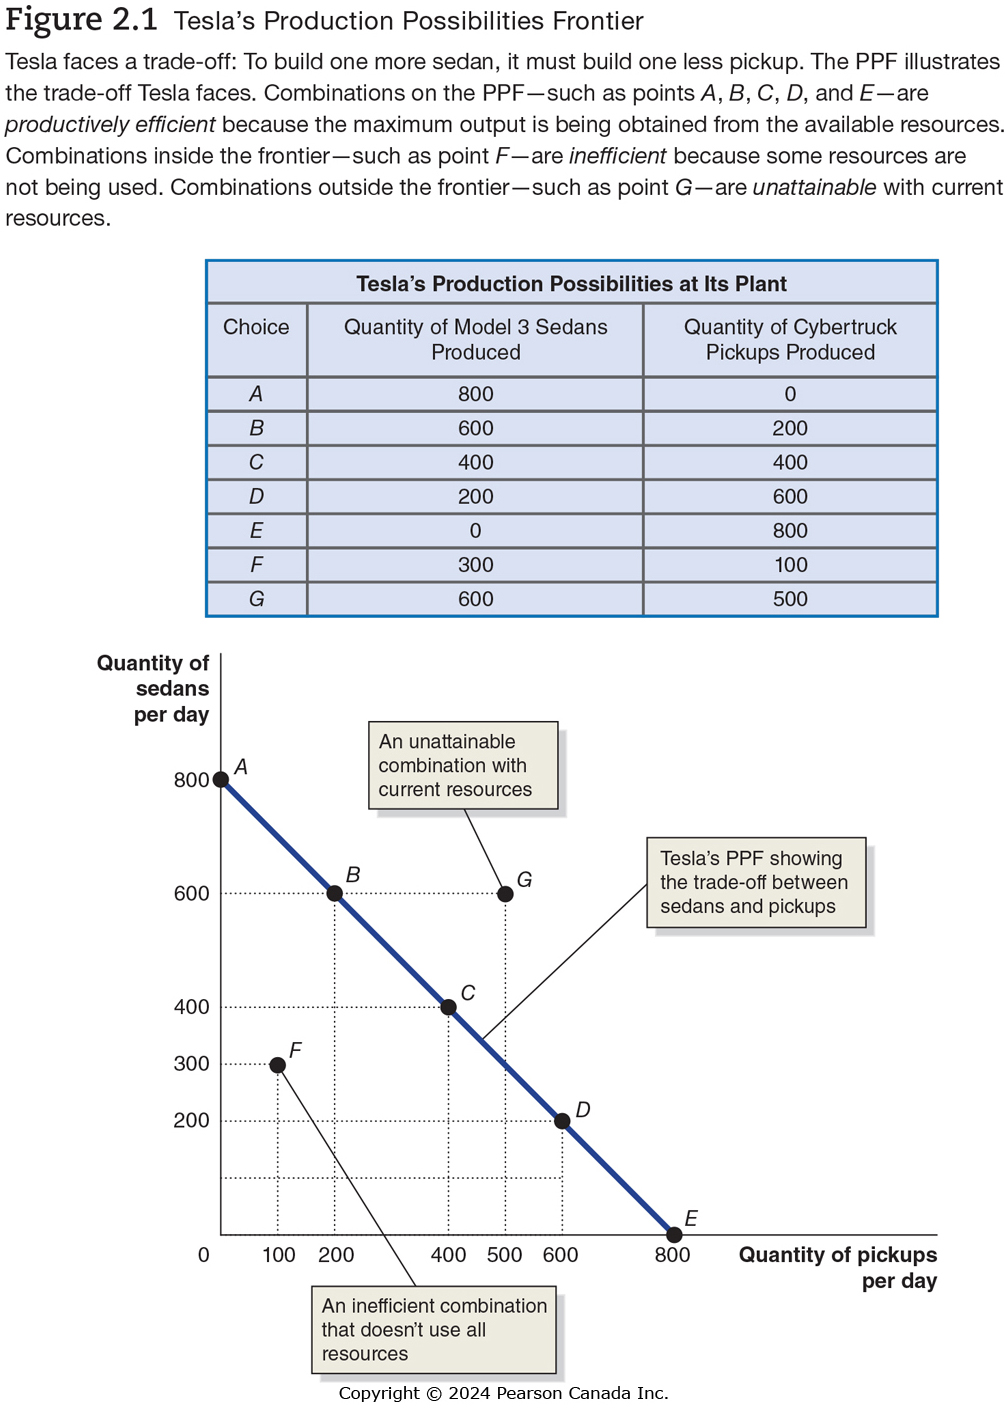
\includegraphics[width=0.3\linewidth]{Fig02-001}.
\end{frame}






\begin{frame}{Interpreting the PPF: Tesla Example}
\transfade
\begin{itemize}[<+->]
  \item Tesla can produce combinations of Model 3 sedans and Cybertruck pickups.
  \item \textbf{Points on} the PPF: attainable and \textbf{productive efficient}.
  \item \textbf{Points below} the PPF: attainable but \textbf{inefficient} (resources underused).
  \item \textbf{Points above} the PPF: currently unattainable with existing resources and technology.
\end{itemize}
\end{frame}

\begin{frame}{Figure 2.1 -- Tesla's PPF and Opportunity Cost (2 of 2)}
\centering
\vspace{2em}

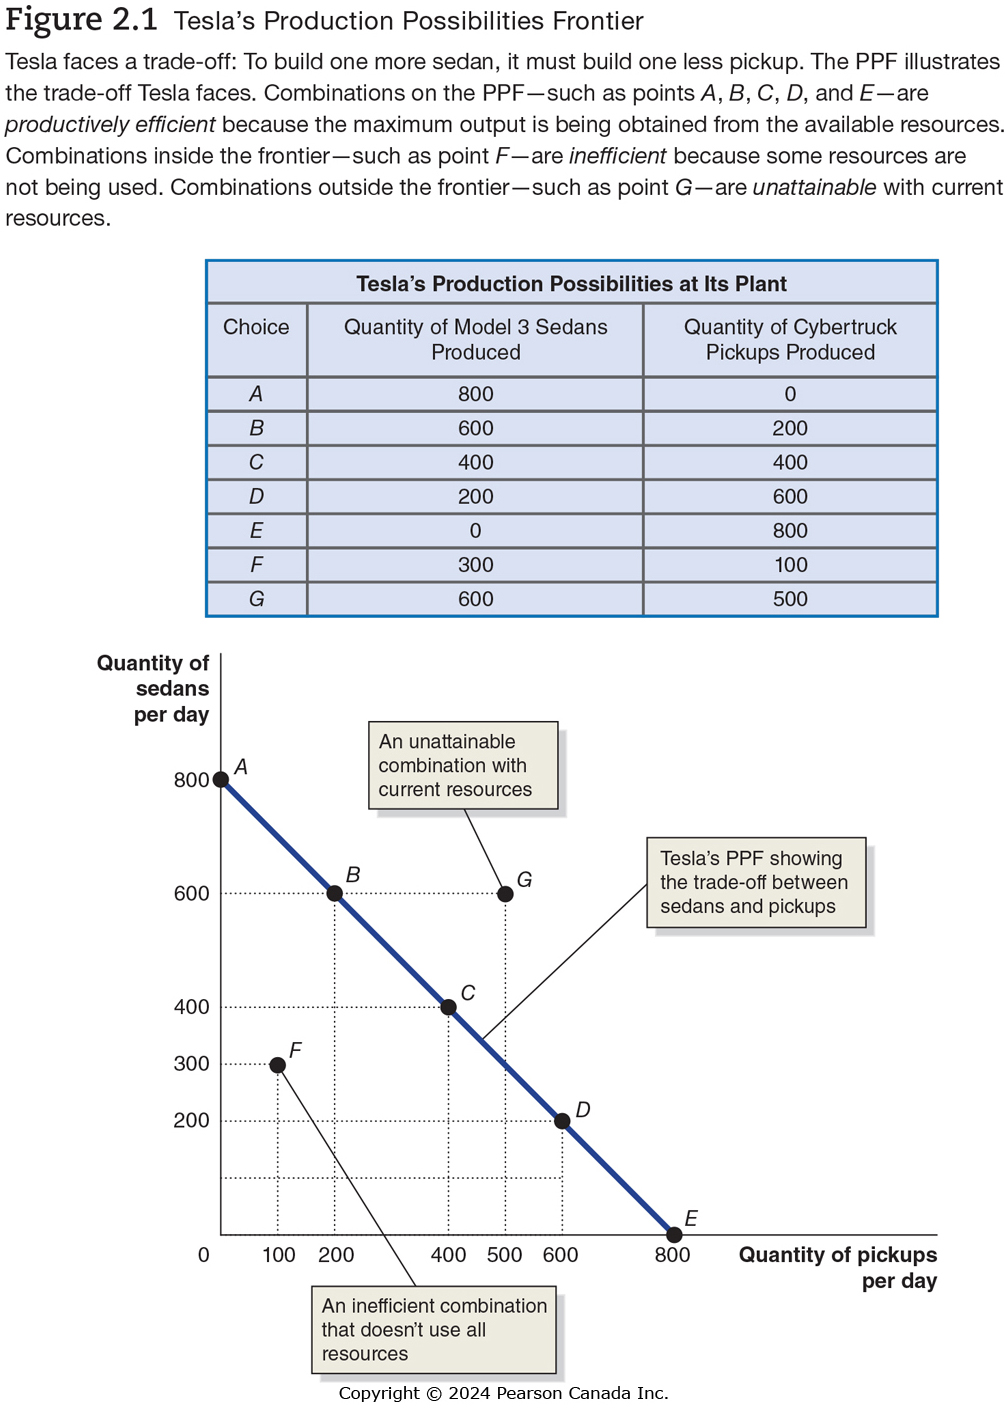
\includegraphics[width=0.3\linewidth]{Fig02-001}.
\end{frame}

\begin{frame}{Opportunity Cost on the PPF}
\transfade
\begin{itemize}[<+->]
  \item Suppose moving from point A to point B:
  \begin{itemize}[<+->]
    \item Tesla produces 200 more Cybertruck pickups.
    \item To do so, it must produce 200 fewer Model 3 sedans.
  \end{itemize}
  \item The \textbf{opportunity cost} of producing 200 more Cybertrucks is the 200 Model 3 sedans given up.
  \item \textbf{Opportunity cost:} the highest-valued alternative that must be given up to engage in an activity.
\end{itemize}
\end{frame}

\begin{frame}{Figure 2.2 -- Increasing Marginal Opportunity Costs}
\centering
\vspace{2em}

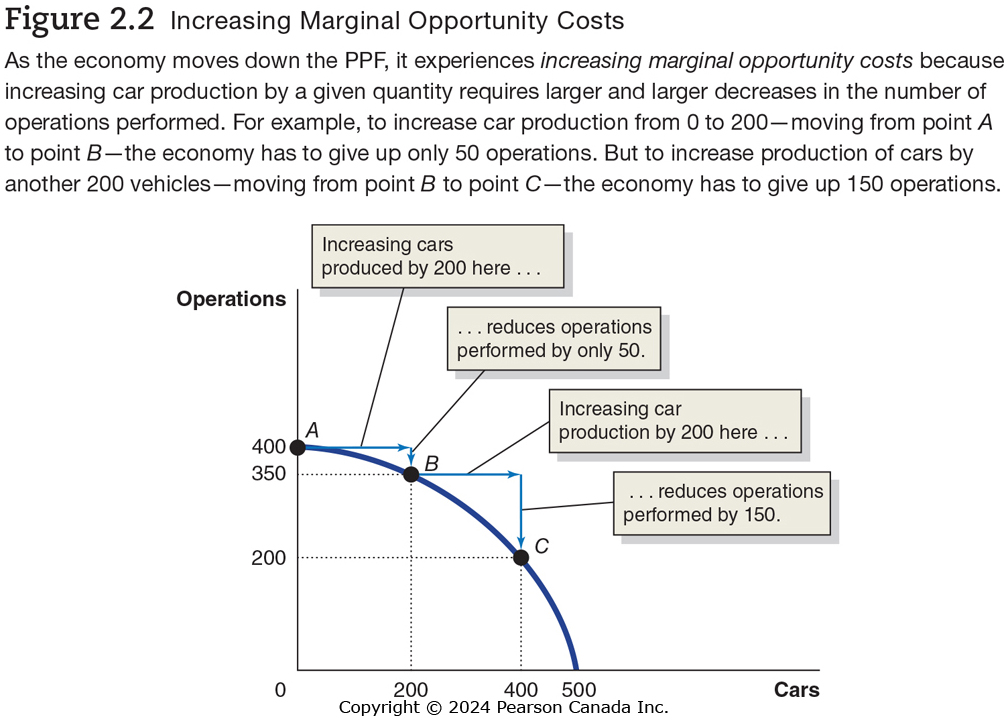
\includegraphics[width=0.6\linewidth]{Fig02-002}.
\end{frame}

\begin{frame}{Why Opportunity Costs Often Increase}
\transfade
\begin{itemize}[<+->]
  \item Some resources are better suited to one task than another.
  \item The first resources to be switched are the ones best suited to switching.
  \item As more resources are devoted to an activity, the extra output from additional resources tends to fall.
  \item This gives the PPF its bowed-out shape and leads to \textbf{increasing marginal opportunity cost}.
\end{itemize}
\end{frame}

\begin{frame}{Figure 2.3 -- Economic Growth}
\centering
\vspace{2em}

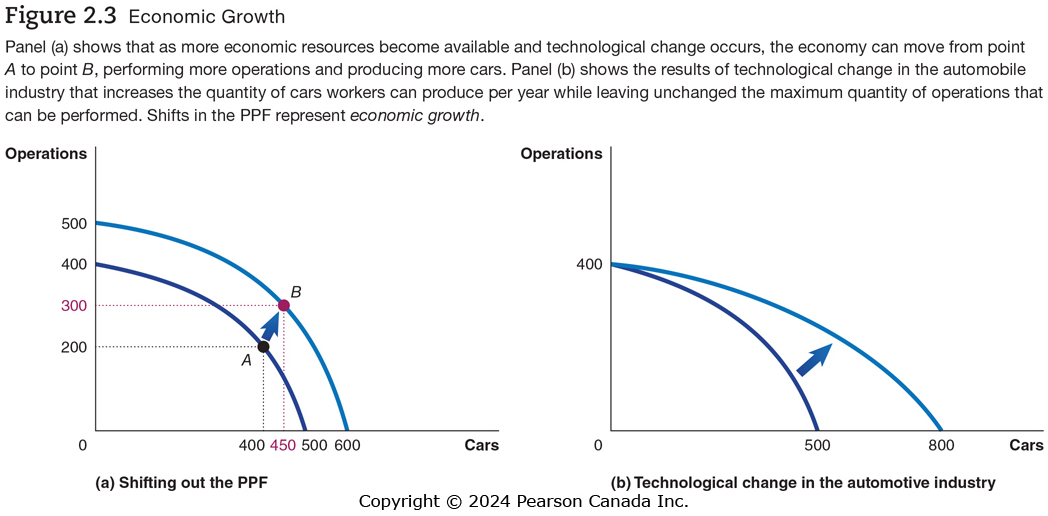
\includegraphics[width=0.8\linewidth]{Fig02-003}.
\end{frame}

\begin{frame}{Economic Growth and the PPF}
\transfade
\begin{itemize}[<+->]
  \item As more economic resources become available, the economy can move from point A to point B, producing more of both goods.
  \item Shifts in the PPF represent \textbf{economic growth}.
  \item \textbf{Economic growth:} the ability of the economy to increase the production of goods and services.
  \item Macro link: long-run growth allows higher living standards without giving up as much of other goods.
\end{itemize}
\end{frame}

\begin{frame}{Figure 2.3 -- Technological Change in One Sector}
\centering
\vspace{2em}

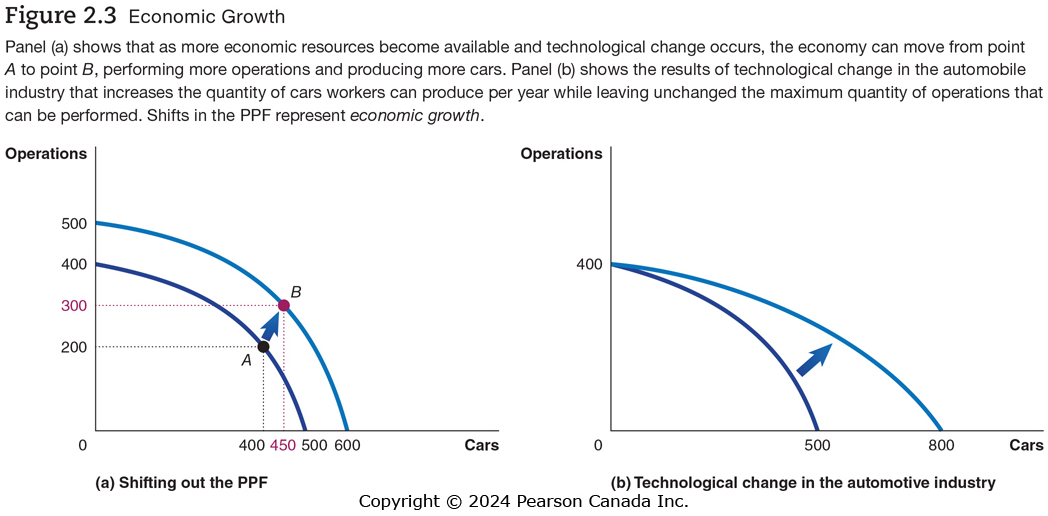
\includegraphics[width=0.8\linewidth]{Fig02-003}.
\end{frame}

\begin{frame}{Technological Change in One Industry}
\transfade
\begin{itemize}[<+->]
  \item Suppose technology improves in the automobile industry only.
  \item The maximum output of automobiles increases, but the production possibility of the other good (e.g., tanks) is unchanged.
  \item Previously unattainable combinations become attainable.
  \item This captures sector-specific technological progress common in macroeconomics (e.g., ICT revolution).
\end{itemize}
\end{frame}

% ============================================================
\section{Comparative Advantage and Trade (2.2)}
% ============================================================

\begin{frame}{2.2 Learning Objective}
\transfade
\begin{block}{Goal}
Understand comparative advantage and explain how it serves as the basis for trade.
\end{block}
\end{frame}

\begin{frame}{Two-Person Production Example: You and Your Neighbour}
\transfade
\begin{itemize}[<+->]
  \item You and your neighbour each have limited time to pick apples and/or cherries.
  \item The table (in the slides) shows:
  \begin{itemize}[<+->]
    \item If you spend all your time picking cherries, you can pick 20 kg of cherries.
    \item If you spend all your time picking apples, you can pick 20 kg of apples.
    \item Your neighbour can pick 60 kg of cherries or 30 kg of apples if she specializes.
  \end{itemize}
  \item We use these numbers to illustrate absolute and comparative advantage.
\end{itemize}
\end{frame}

\begin{frame}{Figure 2.4 -- Production Possibilities for You and Your Neighbour, Without Trade}
\centering
\vspace{2em}

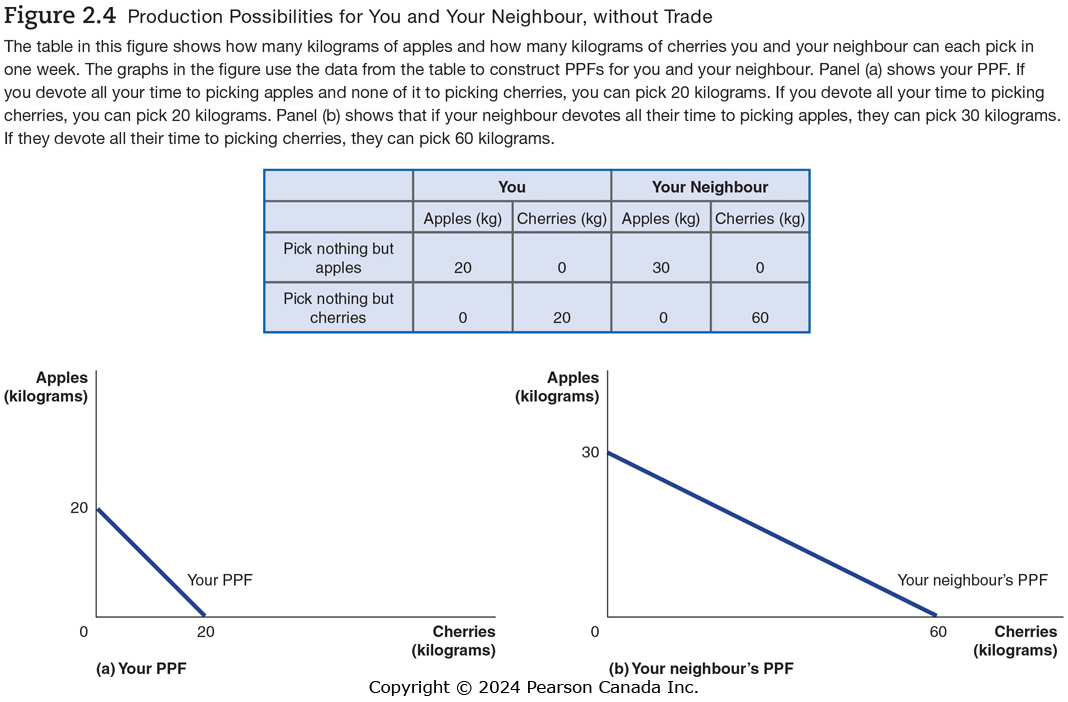
\includegraphics[width=0.58\linewidth]{Fig02-004}.
\end{frame}

\begin{frame}{Autarky (No Trade) Outcomes}
\transfade
\begin{itemize}[<+->]
  \item Without trade, each person consumes only what they produce.
  \item \textbf{You:} pick and consume 8 kg of apples and 12 kg of cherries per week (point A).
  \item \textbf{Neighbour:} picks and consumes 9 kg of apples and 42 kg of cherries per week (point C).
  \item Both are on their own PPFs but may not be at the best possible consumption points if trade is allowed.
\end{itemize}
\end{frame}

\begin{frame}{Specialization and Gains from Trade}
\transfade
\begin{itemize}[<+->]
  \item \textbf{Trade:} the act of buying and selling.
  \item What if you and your neighbour decide to specialize and trade?
  \item Your neighbour appears better at picking both apples and cherries, but:
  \begin{itemize}[<+->]
    \item You can still both benefit from trade by specializing in what you are \textbf{relatively} good at.
  \end{itemize}
\end{itemize}
\end{frame}

\begin{frame}{Figure 2.5 -- Gains from Trade (1 of 2)}
\centering
\vspace{2em}

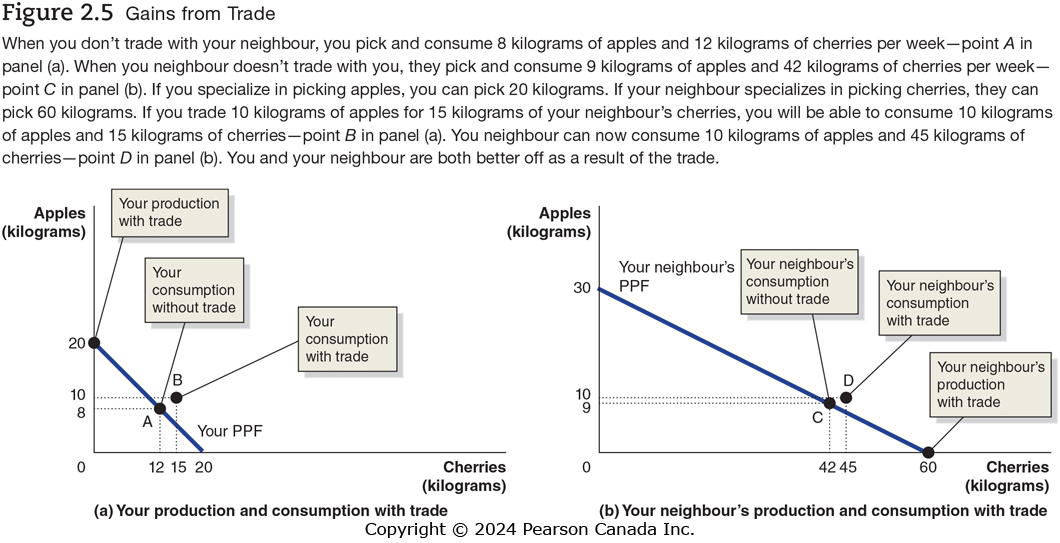
\includegraphics[width=0.8\linewidth]{Fig02-005}.
\end{frame}


\begin{frame}{Numerical Trade Example}
\transfade
\small
\begin{itemize}[<+->]
  \item If you specialize in picking apples, you can pick 20 kg.
  \item If your neighbour specializes in picking cherries, she can pick 60 kg.
  \item Suppose you trade 10 kg of your apples for 15 kg of your neighbour's cherries:
  \begin{itemize}[<+->]
    \item \textbf{You} consume 10 kg of apples and 15 kg of cherries (point B).
    \item \textbf{Neighbour} consumes 10 kg of apples and 45 kg of cherries (point D).
  \end{itemize}
  \item Both are better off than in autarky.
\end{itemize}
\end{frame}

\begin{frame}{Figure 2.5 -- Gains from Trade (2 of 2)}
\centering
\vspace{2em}

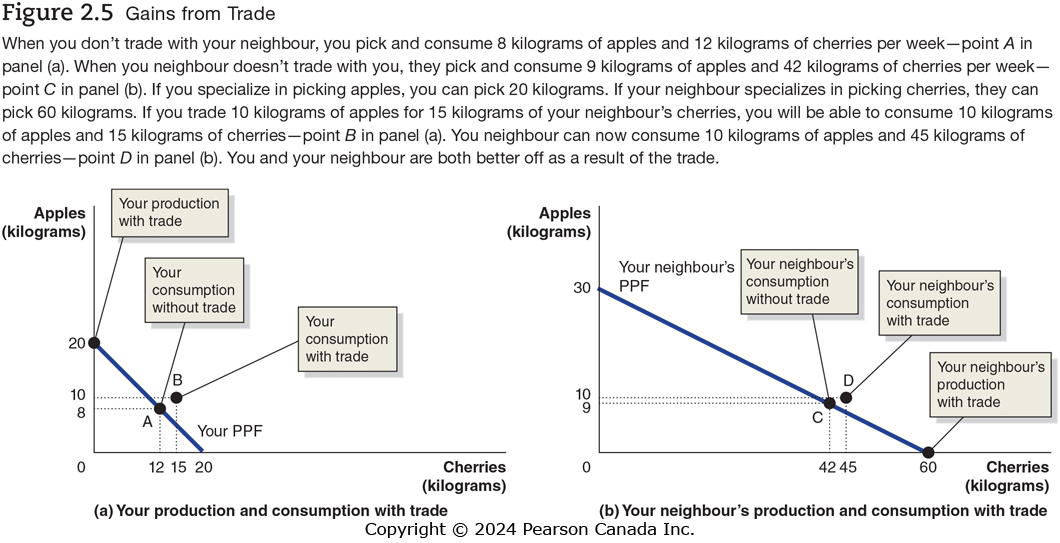
\includegraphics[width=0.8\linewidth]{Fig02-005}.
\end{frame}

\begin{frame}{Table 2.1 -- Summary of the Gains From Trade}
\centering
\vspace{2em}

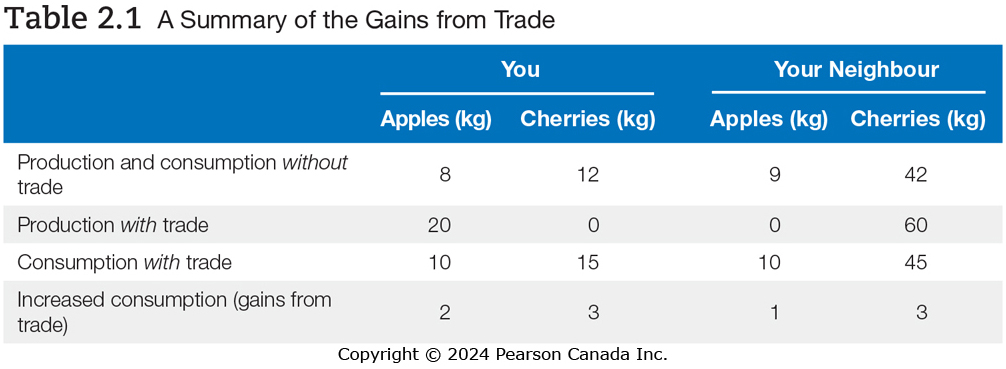
\includegraphics[width=0.99\linewidth]{Tab02-001}.
\end{frame}


\begin{frame}{Table 2.1 -- Summary of the Gains From Trade}
\transfade
\begin{itemize}[<+->]
  \item Both you and your neighbour are able to consume more with trade than without trade.
  \item Key points to emphasize to students:
  \begin{itemize}[<+->]
    \item Trade allows consumption points outside each individual's own PPF.
    \item Even if one person is better at producing \emph{both} goods, both can gain.
  \end{itemize}
\end{itemize}
\end{frame}

\begin{frame}{Explaining the Gains from Trade}
\transfade
\begin{itemize}[<+->]
  \item Your neighbour has an \textbf{absolute advantage} in both cherry and apple picking.
  \item You have a \textbf{comparative advantage} in picking apples.
  \item \textbf{Absolute advantage:} ability to produce more of a good or service than competitors using the same amount of resources.
  \item \textbf{Comparative advantage:} ability to produce a good or service at a lower opportunity cost than competitors.
\end{itemize}
\end{frame}

\begin{frame}{Table 2.2 -- Opportunity Costs of Picking Apples and Cherries}
\centering
\vspace{2em}

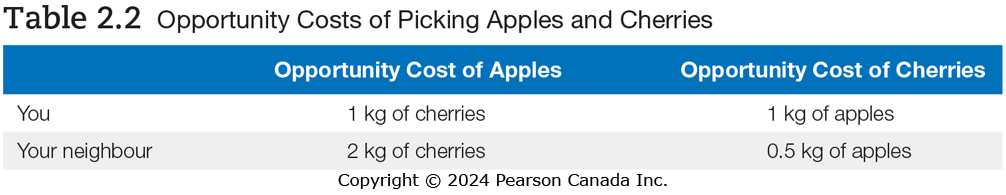
\includegraphics[width=0.99\linewidth]{Tab02-002}.
\end{frame}



\begin{frame}{Table 2.2 -- Opportunity Costs of Picking Apples and Cherries}
\transfade
\begin{itemize}[<+->]
  \item This table compares the opportunity cost of apples vs.\ cherries for you and your neighbour.
  \item The key lesson:
  \begin{itemize}[<+->]
    \item The basis for trade is \textbf{comparative advantage}, not absolute advantage.
    \item Individuals, firms, and countries are better off if they specialize in producing goods and services for which they have a comparative advantage and obtain the other goods and services they need by trading.
  \end{itemize}
\end{itemize}
\end{frame}



% ============================================================
\section{The Market System (2.3)}
% ============================================================

\begin{frame}{2.3 Learning Objective}
\transfade
\begin{block}{Goal}
Explain the basic idea of how a market system works.
\end{block}
\end{frame}

\begin{frame}{Markets and the Modern Economy}
\transfade
\begin{itemize}[<+->]
  \item A \textbf{market} is a group of buyers and sellers of a good or service, and the institution or arrangement by which they come together to trade.
  \item Two key groups participate in the modern economy:
  \begin{itemize}[<+->]
    \item \textbf{Households}
    \item \textbf{Firms}
  \end{itemize}
\end{itemize}
\end{frame}

\begin{frame}{Households and Firms}
\transfade
\begin{itemize}[<+->]
  \item \textbf{Households} consist of individuals who provide the \textbf{factors of production}:
  \begin{itemize}[<+->]
    \item labour, capital, natural resources, and entrepreneurial ability.
  \end{itemize}
  \item Households receive payments for these factors by selling them to firms in \textbf{factor markets}.
  \item \textbf{Firms} supply goods and services to \textbf{product markets}; households buy these products from the firms.
\end{itemize}
\end{frame}

\begin{frame}{The Four Factors of Production}
\transfade
\begin{itemize}[<+->]
  \item \textbf{Labour:} all types of work, from part-time jobs at McDonald\'s to CEOs of large corporations.
  \item \textbf{Capital:} physical capital such as computers, machines, and buildings used to produce other goods.
  \item \textbf{Natural resources:} land, water, oil, iron ore, and other raw materials (``gifts of nature'').
  \item \textbf{Entrepreneur:} someone who operates a business.
  \item \textbf{Entrepreneurial ability:} ability to bring together the other factors of production to produce and sell goods and services successfully.
\end{itemize}
\end{frame}

\begin{frame}{Figure 2.6 -- The Circular-Flow Diagram (1 of 2)}
\centering
\vspace{2em}

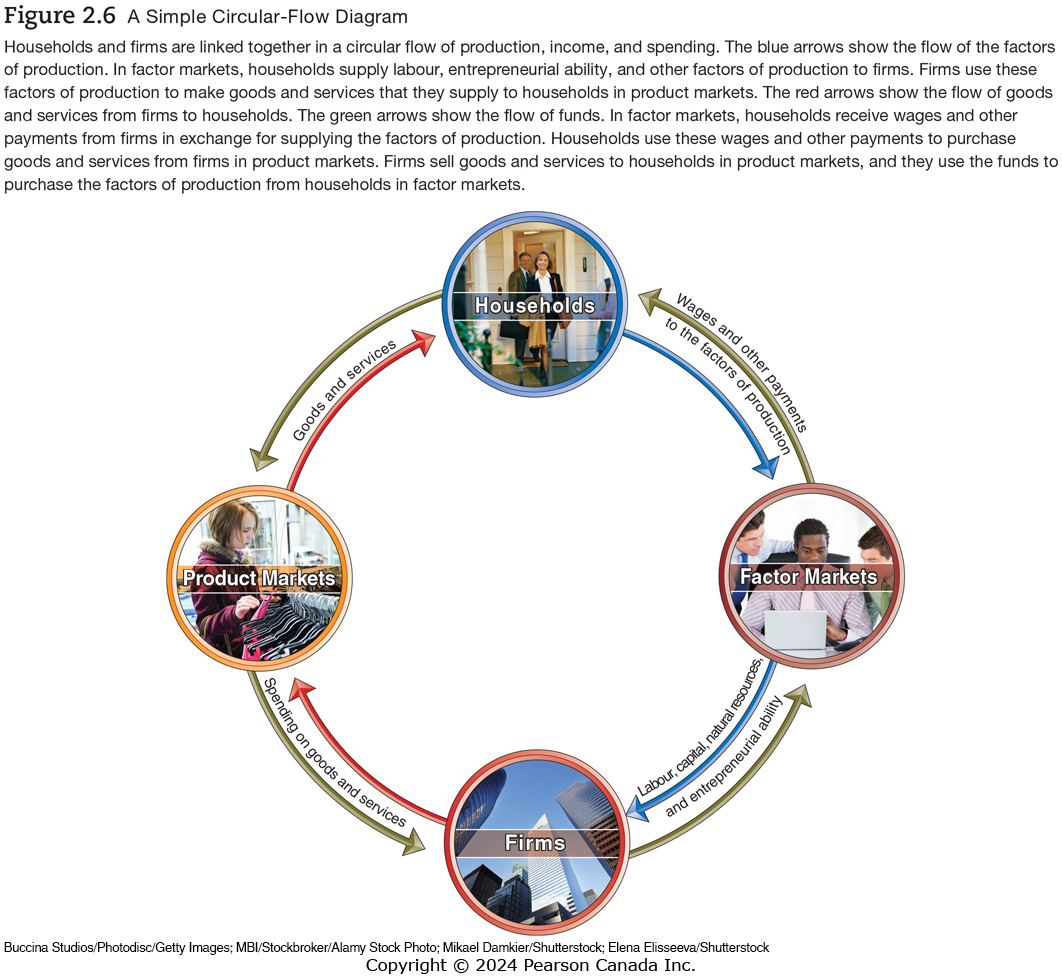
\includegraphics[width=0.5\linewidth]{Fig02-006}.
\end{frame}

\begin{frame}{Circular-Flow Diagram: Basic Idea}
\transfade
\begin{itemize}[<+->]
  \item The \textbf{circular-flow diagram} is a model that illustrates how participants in markets are linked.
  \item \textbf{Real flows:}
  \begin{itemize}[<+->]
    \item Households provide factors of production to firms.
    \item Firms provide goods and services to households.
  \end{itemize}
  \item \textbf{Money flows:}
  \begin{itemize}[<+->]
    \item Firms pay money to households for the factors of production.
    \item Households pay money to firms for goods and services.
  \end{itemize}
\end{itemize}
\end{frame}

\begin{frame}{Figure 2.6 -- The Circular-Flow Diagram (2 of 2)}
\centering
\vspace{2em}

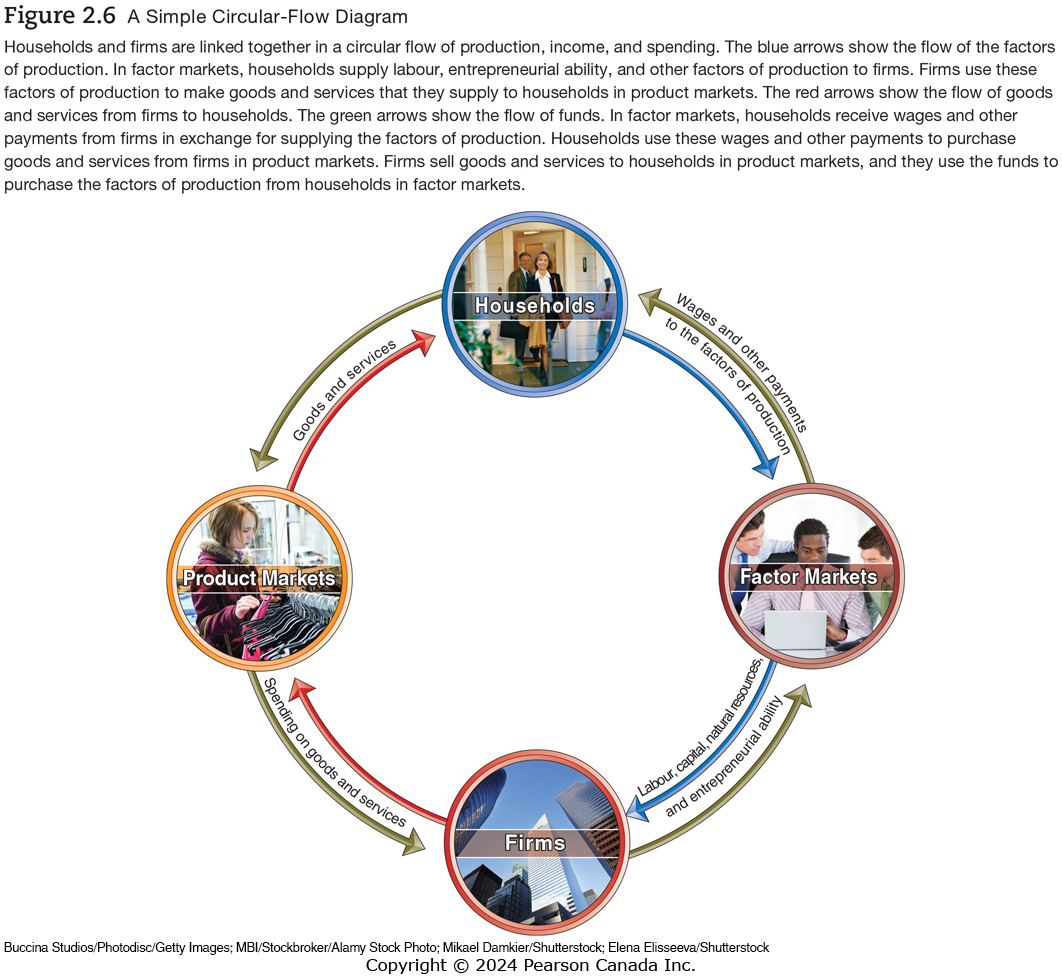
\includegraphics[width=0.5\linewidth]{Fig02-006}.
\end{frame}

\begin{frame}{Limits of the Simple Circular-Flow Model}
\transfade
\begin{itemize}[<+->]
  \item Like all economic models, the circular-flow diagram is a \textbf{simplified} version of reality.
  \item The basic version excludes:
  \begin{itemize}[<+->]
    \item Government
    \item Financial system (banks, credit markets)
    \item Foreign buyers and sellers of goods and services
  \end{itemize}
  \item We add these sectors later in the course to build full macro models.
\end{itemize}
\end{frame}

\begin{frame}{Gains from Free Markets}
\transfade
\begin{itemize}[<+->]
  \item A \textbf{free market} has few government restrictions on:
  \begin{itemize}[<+->]
    \item how goods or services can be produced or sold, or
    \item how factors of production can be employed.
  \end{itemize}
  \item Countries that come closest to this benchmark have typically been more successful than centrally planned economies in raising living standards.
  \item Classic idea: Adam Smith\'s \textbf{``invisible hand''} -- individuals acting in their own self-interest collectively satisfy the wants of consumers.
\end{itemize}
\end{frame}

% ============================================================
\section{Things to Remember \& Chapter Summary}
% ============================================================

\begin{frame}{Things to Remember}
\transfade
\begin{itemize}[<+->]
  \item The production possibilities frontier should \textbf{never bow inward}. Why?
    \begin{itemize}[<+->]
      \item Because opportunity cost typically increases as you move along the PPF.
    \end{itemize}
  \item The PPF tells us what \textbf{can} be produced, not what \textbf{should} be produced.
  \item Just because someone is better or worse at \emph{everything} does not mean trade with them cannot be beneficial.
  \item The basis for trade is \textbf{comparative advantage}, not absolute advantage.
  \item Free markets raise the standard of living, but that does not mean there is no role for governments:
    \begin{itemize}[<+->]
      \item Governments must provide a sound legal environment for the market system to succeed.
    \end{itemize}
\end{itemize}
\end{frame}

\begin{frame}{Summary}
\transfade
\begin{itemize}[<+->]
  \item PPFs illustrate trade-offs, opportunity cost, economic growth, and technological change.
  \item Comparative advantage explains why individuals and countries gain from specialization and trade, even when one side has an absolute advantage in everything.
  \item The market system coordinates decisions of households and firms through product and factor markets.
  \item The circular-flow diagram provides a simple macro picture of how goods, services, and money move in the economy.
  \item Free markets and well-functioning institutions are central to long-run improvements in living standards.
\end{itemize}
\end{frame}

% ============================================================
\begin{frame}
\centering
\Huge \textbf{Thank you!}
\end{frame}

\end{document}
